\def\beginanswers{\iffalse}
%%\def\beginanswers{\iftrue}

\documentclass[10pt]{article}
\usepackage{amsmath,amsfonts,amsthm,amssymb}
\usepackage{graphicx}
\usepackage{enumerate}
\usepackage{upquote,textcomp}
\usepackage{listings}
\usepackage{color}

\definecolor{mygreen}{rgb}{0,0.6,0}
\definecolor{mygray}{rgb}{0.5,0.5,0.5}
\definecolor{mymauve}{rgb}{0.58,0,0.82}


\lstset{frame=tb,
  language=,
  aboveskip=3mm,
  belowskip=3mm,
  showstringspaces=false,
  columns=flexible,
  keepspaces=true,
  basicstyle={\small\ttfamily},
  numbers=none,
  numberstyle=\tiny\color{black},
  keywordstyle=\color{black},
  commentstyle=\color{black},
  stringstyle=\color{black},
  breaklines=true,
  breakatwhitespace=true,
  tabsize=3
}

\lstset{frame=tb,
  language=Python,
  aboveskip=3mm,
  belowskip=3mm,
  showstringspaces=false,
  columns=flexible,
  basicstyle={\small\ttfamily},
  numbers=none,
  numberstyle=\tiny\color{mygray},
  keywordstyle=\color{blue},
  commentstyle=\color{mygreen},
  stringstyle=\color{mymauve},
  breaklines=true,
  breakatwhitespace=true,
  tabsize=3
}


\newcommand{\vect}[1]{{\bf #1}}                 %for bold chars
\newcommand{\vecg}[1]{\mbox{\boldmath $ #1 $}}  %for bold greek chars
\newcommand{\matx}[1]{{\bf #1}}

\setlength{\parindent}{0in}
\setlength{\parskip}{1em}
\setlength{\textheight}{9.5in}
\setlength{\textwidth}{7in}
\setlength{\headsep}{0in}        % distance from top of page to address
\setlength{\topmargin}{-0.5in}
\setlength{\oddsidemargin}{-0.5in}
\setlength{\evensidemargin}{-0.5in}


\begin{document}
\thispagestyle{empty}

\vspace*{0.5in}

\begin{center}
\Large
\textbf{Open Source Software --- CSCI-4966-01 --- Spring 2019} \\
\textbf{Test 1} \\
\textbf{February 22, 2018}
\end{center}


%%%%%%%%%%%%%%%%%%%%%%%%%%%%%%%%%%%%%%%%%%%%%%%%%%%%%%%%%%%%%%%%%%%%%%%%
%%%%%%%%%%%%%%%%%%%%%%%%%%%%%%%%%%%%%%%%%%%%%%%%%%%%%%%%%%%%%%%%%%%%%%%%
\beginanswers
\begin{center}
\Large
\textbf{SOLUTIONS}
\end{center}

%%%%%%%%%%%%%%%%%%%%%%%%%%%%%%%%%%%%%%%%%%%%%%%%%%%%%%%%%%%%%%%%%%%%%%%%
\else
%%%%%%%%%%%%%%%%%%%%%%%%%%%%%%%%%%%%%%%%%%%%%%%%%%%%%%%%%%%%%%%%%%%%%%%%


\begin{center}

\textbf{\Large Name:} \underline {\hspace{2.0in}} \\

\bigskip
\bigskip

\centerline{
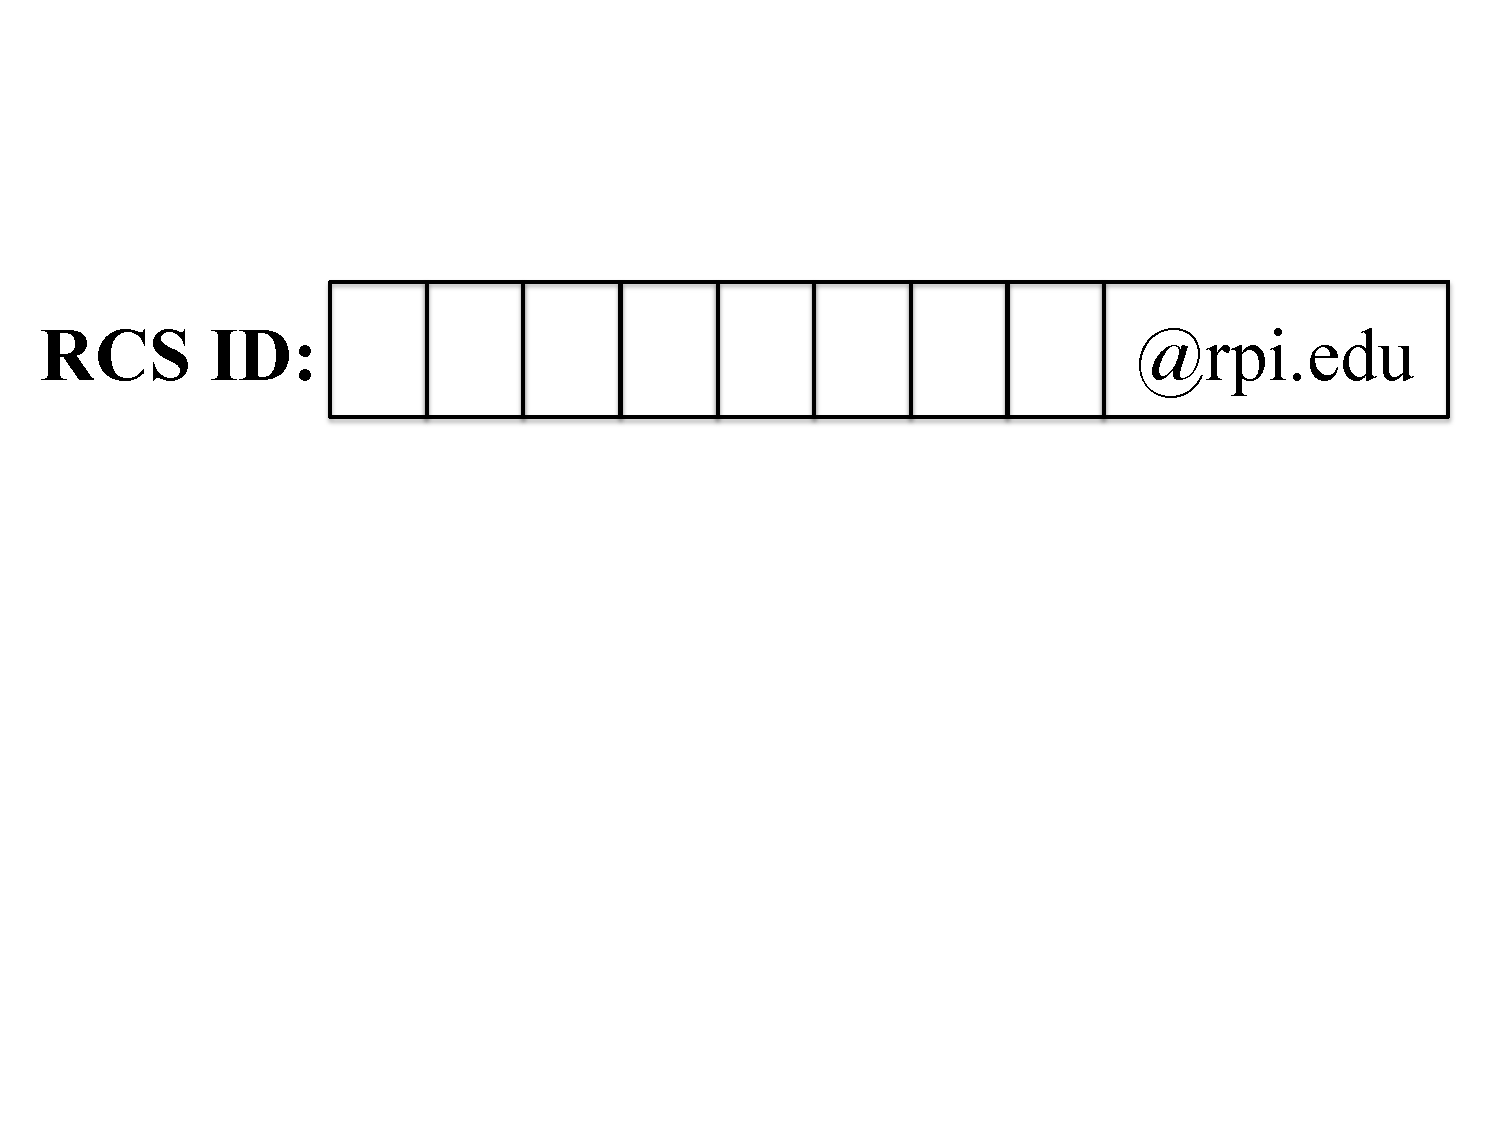
\includegraphics[height=0.5in]{boxes}
}

%%  \begin{tabular}{|p{0.1in}|p{0.1in}|p{0.1in}|p{0.1in}|p{0.1in}|p{0.1in}|p{0.1in}|p{0.1in}|l|}
%%    \hline \\
%%   & & & & & & & & \textbf{\large @rpi.edu} \\
%%  \hline
%%  \end{tabular} 
%%  
%%  \end{tabular}

\bigskip

\textbf{\Large RIN\#:} \underline {\hspace{1.5in}}  

\vspace*{0.4in}
{\large\bf Honor pledge: On my honor I have neither given
nor received aid on this exam.}

\vspace*{0.1in}
{\large\bf Please sign here to indicate that you agree with the honor pledge: \underline {\hspace{1.5in}}}
\end{center}

\vspace*{.45in} 

{\large\bf Instructions:}
\begin{itemize}
%%\item You have 90 minutes to complete this test.
\item Clearly print your name, RCS ID (in all caps.) and your RIN at the top of your exam.
\item This test is open book, open notes and open computer. You {\textbf may not} use the internet. Please turn off your wifi.
%%\item You must {\bf have your Student ID} and you must be seated in the {\bf correct section}. Failure will incur a 
%%{\bf 20 point penalty for each infraction.} If you are unsure if you
%%are in the right section, please see a proctor
%%before the exam starts.
%%\item You may use only one double-sided crib sheet.
%% Put your name and your rcs id on it and turn it in 
%%at the end of the exam.  Otherwise, put
%%  away all books, laptop computers, and electronic devices.
%%\item Please read each question carefully several times before
%%  beginning to work.
%%\item In all the questions, your output must match exactly the given
%%  output (do not insert additional spaces if they are not in the
%%  output).
%%\item We generally will not answer questions except when there is a
%%  glaring mistake or ambiguity in the statement of a question.
%%\item Except for problem 2, there are no Python syntax errors anywhere
%%  on this test. 
%%\item Unless otherwise stated, you may use any valid Python technique to solve any problem.
%%\item Please state clearly any assumptions that you have to make in
%%  interpreting a question.
\item There are \textbf{8 questions} on this test worth a total of
  \textbf{100 points}.
%%\item When you are finished with this test please turn it into one of
%%  the proctors along with your crib sheet.
%%  After you show the proctor your student id you will be free to leave
%%  the exam room.
\end{itemize}

\centering{\begin{tabular}{|c|c|r|}
	\hline
	Question & Score & Possible \\ \hline
	1 &  & 15 \\ \hline
	2 &  & 13 \\ \hline
	3 &  & 12 \\ \hline
	4 &  & 15 \\ \hline
	5 &  & 10 \\ \hline
	6 &  & 15 \\ \hline
	7 &  & 6 \\ \hline
	8 &  & 14 \\ \hline
	Total &  & 100 \\ \hline
\end{tabular}}

\newpage

%%%%%%%%%%%%%%%%%%%%%%%%%%%%%%%%%%%%%%%%%%%%%%%%%%%%%%%%%%%%%%%%%%%%%%%%
\fi
%%%%%%%%%%%%%%%%%%%%%%%%%%%%%%%%%%%%%%%%%%%%%%%%%%%%%%%%%%%%%%%%%%%%%%%%

\begin{enumerate}

	\item The Open Source Initiative defines 10 characteristics of open source software. List 5 along with a \textbf{brief} explanation of what they mean: (15 pts)
	
\beginanswers
Need 5 of the 10 below. Each correct characteristic is worth 3 points with the \textbf{bolded} phrases (or close) worth 1 point. Description is worth 2 points.
\begin{enumerate}
\item \textbf{Free Redistribution}
The license shall not restrict any party from selling or giving away the software as a component of an aggregate software distribution containing programs from several different sources. The license shall not require a royalty or other fee for such sale.
\item \textbf{Source Code}
The program must include source code, and must allow distribution in source code as well as compiled form. Where some form of a product is not distributed with source code, there must be a well-publicized means of obtaining the source code for no more than a reasonable reproduction cost, preferably downloading via the Internet without charge. The source code must be the preferred form in which a programmer would modify the program. Deliberately obfuscated source code is not allowed. Intermediate forms such as the output of a preprocessor or translator are not allowed.
\item \textbf{Derived Works}
The license must allow modifications and derived works, and must allow them to be distributed under the same terms as the license of the original software.
\item \textbf{Integrity of The Author's Source Code}
The license may restrict source-code from being distributed in modified form only if the license allows the distribution of "patch files" with the source code for the purpose of modifying the program at build time. The license must explicitly permit distribution of software built from modified source code. The license may require derived works to carry a different name or version number from the original software.
\item \textbf{No Discrimination Against Persons or Groups}
The license must not discriminate against any person or group of persons.
\item \textbf{No Discrimination Against Fields of Endeavor}
The license must not restrict anyone from making use of the program in a specific field of endeavor. For example, it may not restrict the program from being used in a business, or from being used for genetic research.
\item \textbf{Distribution of License}
The rights attached to the program must apply to all to whom the program is redistributed without the need for execution of an additional license by those parties.
\item \textbf{License Must Not Be Specific to a Product}
The rights attached to the program must not depend on the program's being part of a particular software distribution. If the program is extracted from that distribution and used or distributed within the terms of the program's license, all parties to whom the program is redistributed should have the same rights as those that are granted in conjunction with the original software distribution.
\item \textbf{License Must Not Restrict Other Software}
The license must not place restrictions on other software that is distributed along with the licensed software. For example, the license must not insist that all other programs distributed on the same medium must be open-source software.
\item \textbf{License Must Be Technology-Neutral}
No provision of the license may be predicated on any individual technology or style of interface.
\end{enumerate}
\else
	\begin{enumerate}[1]
	\bigskip
	\item -
	\bigskip
	\bigskip
	\bigskip
	\bigskip
	\bigskip
	\item -
	\bigskip
	\bigskip
	\bigskip
	\bigskip
	\bigskip
	\item -
	\bigskip
	\bigskip
	\bigskip
	\bigskip
	\bigskip
	\item -
	\bigskip
	\bigskip
	\bigskip
	\bigskip
	\bigskip
	\item -
	\bigskip
	\bigskip
	\bigskip
	\bigskip
	\bigskip
\end{enumerate}
\fi

\item Consider the scenario where a company is using open source software to produce applications that they then sell. 
\begin{enumerate}
\item What is the impact (license, ability to distribute, etc.) on their product if the open source software they used is licensed under:  (9 pts)
	
\beginanswers
\begin{enumerate}
\item GPL:
Any code that is distrbuted (given away or sold) and that directly uses or links to GPL code must be licensed under the GPL or a compatible license.
\bigskip
\item LGPL:
Any code that is distrbuted (given away or sold) and that directly uses or \textbf{staticly} links to the LGPL code must be licensed under the LGPL or a compatible license. The idea here is that if the LGPL code can be modified and those modifications then used in the distributed product, the terms of the LGPL are met. That is why dynamic linking is allowed but not static linking.
\bigskip
\item MIT:
Any code that is distrbuted (given away or sold) and that directly uses or links to the MIT licensed code must carry copyright and license notice for the original work.
\bigskip
\end{enumerate}
\else
\begin{enumerate}
	\item GPL:
	\bigskip
	\bigskip
	\bigskip
	\bigskip
	\bigskip
	\item LGPL:
	\bigskip
	\bigskip
	\bigskip
	\bigskip
	\bigskip
	\item MIT:
	\bigskip
	\bigskip
	\bigskip
	\bigskip
	\bigskip
	\end{enumerate}
\fi
\item Which license (in the open source software they are using) serves the company best if their business plan is to (4 pts):
\beginanswers
\begin{enumerate} 
	\item Sell unique software that they developed which uses the Open Source Software
	\bigskip
	
	MIT - 
	
	Under the MIT license, they are free to license any changes they make according to whatever business plan they choose. They may even make the resulting software product proprietary so long as they include the original copyright and license notices when distributing the software.
	\bigskip
	\item Provide support services around the Open Source Software they are using without creating new applications or code
		\bigskip
	
	GPL - 
	
	The company is not basing their business plan and ability to compete on any software differentiators. Instead they are competing based on service. The GPL ensures that any competitor cannot``outflank'' them by making proprietary changes to the software that makes the competing version  ``better.'' Instead, the GPL requires that all such changes be disclosed keeping the competition for customers solely on the services provided.
	\bigskip
\end{enumerate}
\else
\begin{enumerate} 
	\item Sell unique software that they developed which uses the Open Source Software
	\bigskip
	\bigskip
	\bigskip
	\bigskip
	\bigskip
	\bigskip
	\bigskip
	\bigskip
	\item Provide support services around the Open Source Software they are using without creating new applications or code
	\bigskip
	\bigskip
	\bigskip
	\bigskip
	\bigskip
	\bigskip
	\bigskip
	\bigskip
\end{enumerate}
\fi
Make sure you support your answer.
\end{enumerate}

\item For each question below, circle the best answer (12 pts)
\beginanswers
\begin{enumerate}
	\item Which command changes you repository to a new (existing) branch?
	\begin{enumerate}
		\item git checkout newbranch
	\end{enumerate}
	\item Literate programming:
	\begin{enumerate}
		\item Mixes code and comments in an easily human readable format
	\end{enumerate}
	\item Open or Free software:
	\begin{enumerate}
		\item Can be redistributed either for free or for a fee
	\end{enumerate}
	\item It is a good idea when selecting an open source license to:
	\begin{enumerate}
		\item Go to an authority such as the OSI and pick an approved license
	\end{enumerate}
\end{enumerate}
\else
\begin{enumerate}
	\item Which command changes you repository to a new (existing) branch?
	\begin{enumerate}
		\item git branch
		\item git status
		\item git checkout newbranch
		\item git log
	\end{enumerate}
 	\item Literate programming:
 	\begin{enumerate}
 		\item Is well structured code with minimal comments
 		\item Cannot express complicated algorithms
 		\item Mixes code and comments in an easily human readable format
 		\item Is a failed development methodology
 	\end{enumerate}
 	\item Open or Free software:
 	\begin{enumerate}
 		\item Cannot be used for a commercial purpose
 		\item Can be redistributed either for free or for a fee
 		\item Can be sold, but only for the nominal cost of the media used to store it
 		\item Must be maintained by unpaid volunteers
 	\end{enumerate}
 	\item It is a good idea when selecting an open source license to:
	\begin{enumerate}
		\item Go to an authority such as the OSI and pick an approved license
		\item Create a new license from scratch because it is unlikely that an existing license would meet your needs
		\item Just place the code in a public repository. Easily available code is the same as open
		\item Take an existing, approved license and modify to better represent your unique personality
	\end{enumerate}
\end{enumerate}
\fi
\newpage
\item Give a sequence of git commands to accomplish the following (you can assume that you are always working on the ``master'' branch'') (15 pts):
\begin{enumerate}
	\item Create a local copy of your repoository by cloning from ``https://www.mypublicrepository/public.git''. This will be your origin.
	\item Create an ``upstream'' remote to point to ``https://www.everyonespublicrepository/public.git''
	\item Assume you have a new file ``foo.txt'' in your local directory. Add this file to your repository.
	\item Send your changes to the public repository
	\item Assume someone else makes changes in the ``upstream''.  Add the changes in the public repository into your local version. 
\end{enumerate}
\bigskip
Write git commands below:
\beginanswers
\begin{lstlisting}
git clone https://www.mypublicrepository/public.git
git remote add upstream https://www.everyonespublicrepository/public.git
git add foo.txt
git commit -m "adding foo"
git push origin master
git pull upstream master
\end{lstlisting}\else
\hspace*{-0.4in}\framebox(540,300){}
\fi
\newpage

\item Write markdown to duplicate the document below. You can assume the photo name is ``photo.jpg'' (10 pts):
\begin{figure}[h]
\centering
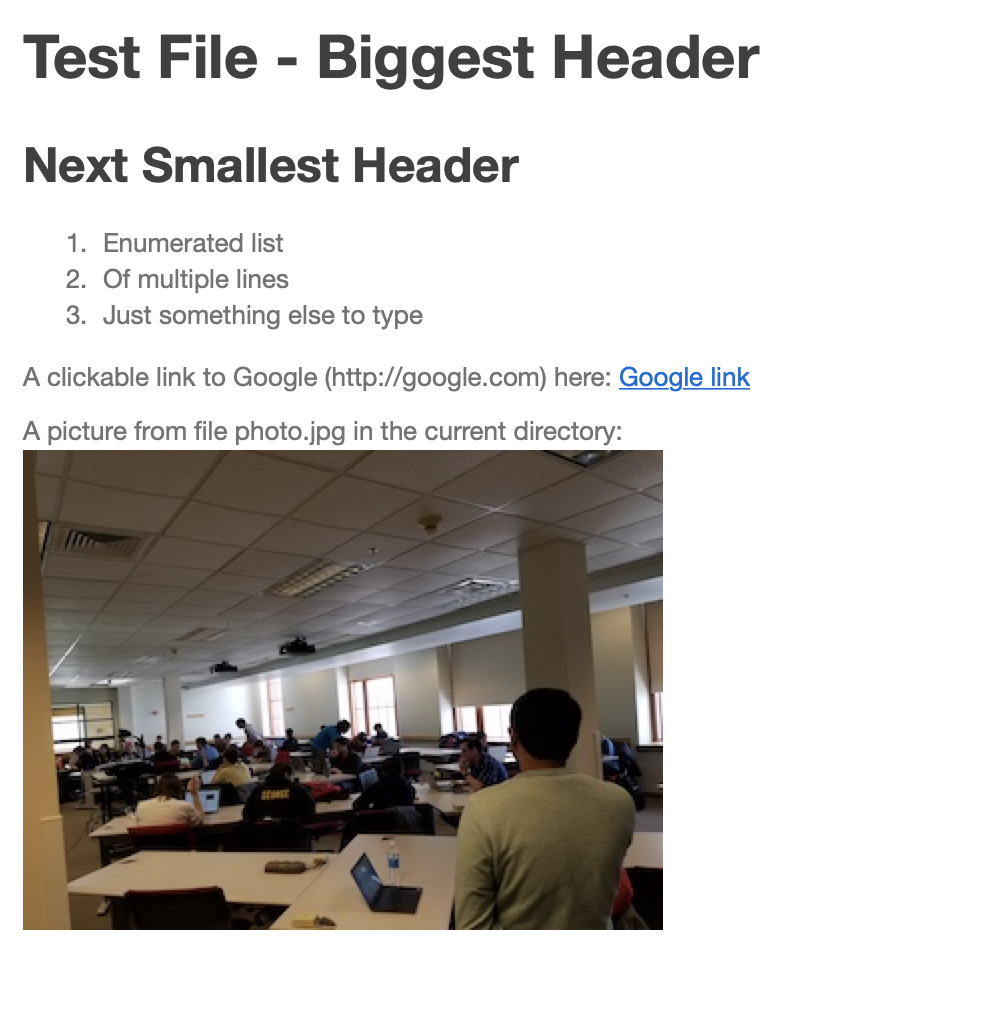
\includegraphics[width=0.6\linewidth]{./test_markdown}
\label{fig:testmarkdown}
\end{figure}

\bigskip
Write Markdown commands below:

\beginanswers

\begin{lstlisting}
# Test File - Biggest Header

## Next Smallest Header

1. Enumerated list
2. Of multiple lines
3. Just something else to type

A clickable link to Google (http://google.com) here: [Google link](http://google.com)

A picture from file photo.jpg in the current directory:
![](./photo.jpg)
\end{lstlisting}
\else
\hspace*{-0.4in}\framebox(540,300){}
\fi
\newpage

\item Assume you have 3 source files: a main file ``prog.c'' and two additional files``f1.c'', and ``f2.c'' containing code that ``prog'' depends upon. Write a Makefile that explicitly creates object files for all 3 sources, create a static library from the ``f1.c'' and ``f2.c'' object files, and then create an executable named ``prog.exe''. Make sure your Makefile contains appropriate ``all'' and ``clean'' targets. (15 pts):
\bigskip

Write your Makefile below:
\beginanswers
\begin{lstlisting}
all: prog.exe

clean:
	rm *.o prog libf.so

prog.exe: prog.o libf.a
	cc -o prog.exe prog.o libf.a

prog.o: prog.c
	cc -c prog.c -o prog.o

libf.a: f1.o f2.o
	ar -qc libf.a f1.o f2.o 
	
f1.o: f1.c
	cc -c f1.c -o f1.o

f2.o: f2.c
	cc -c f2.c -o f2.o
\end{lstlisting}
or
\begin{lstlisting}
all: prog.exe

clean:
	rm *.o prog.exe libf.a

prog.exe: prog.o libf.a
	cc -o prog.exe prog.o libf.a

prog.o: prog.c

libf.a: f1.o f2.o
	ar -qc libf.a f1.o f2.o

f1.o: f1.c

f2.o: f1.c
\end{lstlisting}
	
\else
\hspace*{-0.4in}\framebox(540,275){}
\fi

\item Repeat the previous exercise for CMake.  (6 pts):
\bigskip
Write your CMakeLists.txt file below:
\beginanswers
\begin{lstlisting}
cmake_minimum_required(VERSION 3.0)
project(Hello C)

add_library(Lib STATIC f1.c f2.c)

add_executable(prog.exe	prog.c)

target_link_libraries(prog.exe Lib)
\end{lstlisting}
\else
\hspace*{-0.4in}\framebox(540,275){}
\fi

\newpage

\item Consider the following code binary search code in file binary.py:
\begin{lstlisting}
def binary_search( x, L):
    low = 0
    high = len(L)
    while low != high:
        mid = (low+high)//2
        if x >= L[mid]:
            low = mid+1
        else:
            high = mid
    return low
\end{lstlisting}
\bigskip

The code contains an error.

\begin{enumerate}
	\item Find and correct the error. Write your correction alongside the code above. You may use any tools on your computer to help you find the error. (2 pts)
\beginanswers
\begin{lstlisting}
def binary_search( x, L):
    low = 0
    high = len(L)
    while low != high:
        mid = (low+high)//2
        if x > L[mid]:
            low = mid+1
        else:
            high = mid
    return low
\end{lstlisting}
\fi
	
	\item Now, on the next page, write a sequence of tests in file binary\_unit\_test.py to ensure that the algorithm is correct. For full credit you will need to cover at least 4 different use cases. We give you the start and the end of the test file (12)
\end{enumerate}
\newpage
\begin{lstlisting}
'''
Test binary.py with unittest
To run tests:
python binary_unit_test.py
'''
import unittest
from binary import binary_search

class TestBinaryPy(unittest.TestCase):

    def setUp(self):
        pass
\end{lstlisting}
\beginanswers
\begin{lstlisting}
    #
    # Pick 4 test cases from the following:
    #
    def test_null(self):
        print("Test the empty list")
        self.assertEqual(binary_search(-5, []), 0)

    def test_before(self):
        print("Test before front")
        self.assertEqual(binary_search(-5, range(0, 15)), 0)

    def test_first(self):
        print("Test at front")
        self.assertEqual(binary_search(0, range(0, 15)), 0)

    def test_after(self):
        print("Test beyond end")
        self.assertEqual(binary_search(15, range(0, 15)), 15)

    def test_last(self):
        print("Test at end")
        self.assertEqual(binary_search(14, range(0, 15)), 14)

    def test_duplicates(self):
        print("Test duplicates")
        self.assertEqual(binary_search(12, 10*[12]), 0)

    def test_middle(self):
        print("Test middle")
        self.assertEqual(binary_search(11, range(0, 15)), 11)
\end{lstlisting}
\else
\hspace*{-0.4in}\framebox(540,450){}
\fi
\begin{lstlisting}
if __name__ == '__main__':
    unittest.main()
\end{lstlisting}

\end{enumerate}
\end{document}

